\question

Con el paquete \mintinline{latex}|booktabs|, es posible crear tablas
tipográficamente sofisticadas.
La documentación ofrece numerosos consejos de diseño y ejemplos de
buenas prácticas.
Lamentablemente, la siguiente tabla no cumple plenamente con estas
recomendaciones.
\begin{table}[ht!]
	\centering
	\begin{tabular}{|p{2.1cm}||p{2.5cm}|cl|lr|}
		\hhline{=-----}
		Produkt      & Herkunft    & Saisonbeginn & Saisonende & Handelsklasse & verfügbar \\\hhline{======}
		Auberginen   & Frankreich  & Juli         & September  & I             & -         \\\hline
		Esskastanien & Frankreich  & September    & September  & I             & -         \\\hline
		Feldsalat    & Deutschland & Oktober      & Februar    & II            & ja        \\\hline
		Kürbis       & Deutschland & August       & Dezember   & I             & ja        \\\hline
		Rote Beete   & Italien     & September    & Februar    & I             & ja        \\\hline
		Zucchini     & Spanien     & Juni         & Oktober    & II            & -         \\\hline
		Zwiebeln     & Deutschland & Mai          & Oktober    & -             & -         \\\hhline{======}
	\end{tabular}
\end{table}

\begin{parts}
	\part

	Corrija esta deficiencia y transfiera la tabla a un documento
	\LaTeX{} según las normas del sector.
	Considere las posibilidades del paquete
	\mintinline{latex}|multirow| y el comando
	\mintinline{latex}|\multicolumn| presentado en la lección.

	\part

	Coloque la tabla en un entorno flotante adecuado y asígnele un
	título descriptivo.

	\part

	Escriba un breve comentario sobre los cambios realizados (motivo de
	los cambios, problemas, soluciones alternativas, etc.).
\end{parts}

\begin{solution}
	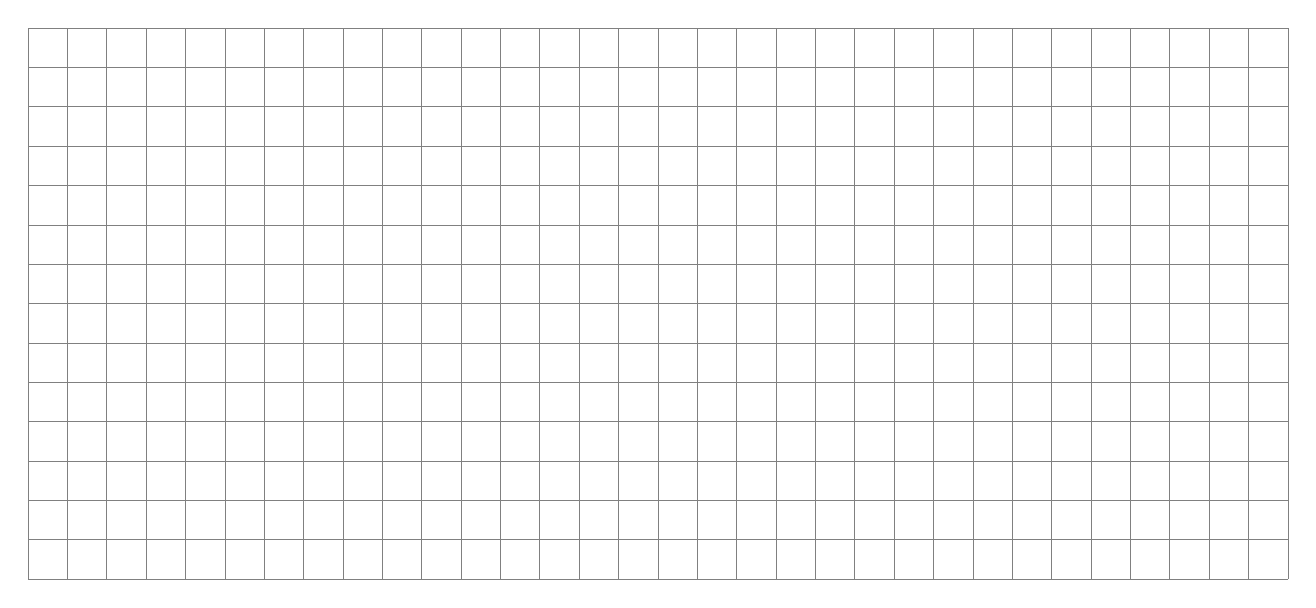
\begin{tikzpicture}[xscale=0.5,yscale=0.5]
		\draw[help lines] (0,0) grid (32,14);
	\end{tikzpicture}
\end{solution}
